\input{preamble}

\title{Computing architectures Part 2}
\institute{NTNU, IMF}
\date{January 26. 2018}
%\author{Aurélien Larcher}
\maketitle

\begin{frame}
  \frametitle{Supercomputing}

\begin{center}
What is the motivation for Supercomputing?
\end{center}

\vspace{2ex}

Solve complex problems fast and accurately:
\begin{itemize}
\item efforts in modelling and simulation push sciences and engineering applications forward,
\item computational requirements drive the development of new hardware and software.
\end{itemize}

\medskip
$\rightarrow$ architectures and software models evolved with the algorithms.

\end{frame}

%----------------------------------------
\begin{frame}
  \frametitle{Supercomputers at NTNU: History}

Supercomputing center established in 1983.
  \begin{center}
    \scalebox{0.8}{
      \input{\data/history}
    }
  \end{center}

\medskip
$\rightarrow$ representative of the evolution of supercomputers

\end{frame}


%----------------------------------------
\begin{frame}
  \frametitle{Evolution: system architecture}

\begin{minipage}[bc]{0.4\linewidth}
\centering
\begin{figure}
\centering
\includegraphics[width=\linewidth]{top500/architecture/Architecture_System}
\end{figure}
\end{minipage}
\begin{minipage}[bc]{0.4\linewidth}
\centering
\begin{figure}
\centering
\includegraphics[width=\linewidth]{top500/architecture/Architecture_Performance}
\end{figure}
\end{minipage}

\smallskip
Comparison of the evolution w.r.t system and performance share.
\end{frame}

%----------------------------------------
\begin{frame}
  \frametitle{Supercomputers}
  \begin{itemize}
  \item 70's--80's: vector processors (CRAY-1 1976); \\
    one or a few expensive, custom-made chips.
  \item 80's--: MPP systems, Constellations; \\
    many processors; standard micro-processors but possibly proprietary interconnects.
  \item Current trend: multicore systems; \\
    heterogeneous computing.
  \end{itemize}

$\rightarrow$ chosen solutions are a compromise between requirements and costs.

\end{frame}

%----------------------------------------
\begin{frame}
  \frametitle{Flynn's Taxonomy}
\begin{table}[h!]
\centering
\caption{Flynn's taxonomy:}
\label{tab:doc}
\begin{tabular}{|c|l|l|}
  \hline
  \hfill & \texttt{SD} & \texttt{MD} \\
  \hline
  \texttt{SI} & Von Neumann (single-processor) & SIMD (vector processors) \\
  \texttt{MD} & \hfill                         & MIMD (multiprocessors) \\
  \hline
\end{tabular}
\end{table}
\medskip
\textit{grain-size}: amount of computation performed by a parallel task.\\
$\rightarrow$ granularity influences the choice of a solution.

  \begin{itemize}
  \item SISD: ILP, memory hierarchy
  \item SIMD: DLP, fine-grained parallelism
  \item MIMD: TLP, coarse-grained parallelism
  \end{itemize}

\end{frame}

\begin{frame}
  \frametitle{Multi-processor systems}
  Challenges:
  \begin{itemize}
  \item communication between processors \\
    (memory access, programming models);
  \item computational methods or algorithms;
  \item scalability (hardware and algorithms);
  \item large volumes of data (storage and visualization).
  \end{itemize}
\end{frame}

%----------------------------------------
\begin{frame}
  \frametitle{Memory hierarchy}
  \begin{center}
    \scalebox{0.8}{
      \input{\figs/tma4280/memory-hierarchy}
    }
  \end{center}

The same bottleneck applies to multiprocessors: different memory architectures and interconnect topologies are developed to overcome the limitations.

\end{frame}

\begin{frame}
  \frametitle{Shared memory access}
  \begin{center}
    \input{\figs/tma4280/global-memory-access}
  \end{center}
\end{frame}

\begin{frame}
  \frametitle{Distributed memory access}
  \begin{center}
    \input{\figs/tma4280/distributed-memory-access}
  \end{center}
\end{frame}

\begin{frame}
  \frametitle{Shared memory: uniform access}
  This is called a \emph{symmetric multi-processor}. Examples: bus-based,
  switch-based and crossbar organizations. Challenges: cache coherency and cost.
  \begin{center}
    \scalebox{0.6}{\input{\figs/tma4280/crossbar}}
  \end{center}
\end{frame}

\begin{frame}
  \frametitle{Shared memory: non-uniform access}
  This is called NUMA or ccNUMA (\emph{cache-coherent non-uniform memory
    access}). Example: Several SMPs connected with a high-speed low-latency
  network. Each SMP has uniform memory access internally.
  \begin{center}
    \input{\figs/tma4280/ccnuma}
  \end{center}
\end{frame}

\begin{frame}
  \frametitle{Distributed memory systems}
  Only the local address space is available to each processor. Data from other
  processors are only available through explicit message-passing.
  \begin{center}
    \input{\figs/tma4280/distributed-memory-computer}
  \end{center}
\end{frame}

\begin{frame}
  \frametitle{Network topology}
  Examples: 2D mesh or toroid. Vilje is an eight-dimensional hyper-cube (!).
  \begin{center}
    \begin{tikzpicture}
  \foreach \i in {0,...,10} {
    \draw[very thick] (\i,0) -- (\i,10);
    \draw[very thick] (0,\i) -- (10,\i);
  }
  \foreach \i in {0,...,3} {
    \foreach \j in {0,...,3} {
      \draw[thick, darkblue, fill=cadet] (\i,\j) circle (0.1);
    }
  }
\end{tikzpicture}

    \qquad
    \input{\figs/tma4280/toroid}
  \end{center}
\end{frame}

\begin{frame}
  \frametitle{The current supercomputer at NTNU}
  Based on the Intel Sandy Bridge microprocessor, an octa-core chip (image
  shows the quad-core version)
  \begin{center}
    \includegraphics[width=9.5cm]{\figs/tma4280/sandy}
  \end{center}
\end{frame}

\begin{frame}
  \frametitle{The current supercomputer at NTNU}
  Intel Sandy bridge E5-2670:
  \begin{itemize}
  \item An octa-core chip (8 physical processing cores)
  \item Caches and memory:
    \begin{itemize}
    \item private L1 cache (32kB instruction+32kB data) 3 clocks;
    \item private L2 cache (256kB) 8 clocks;
    \item shared L3 cache (20MB) $\sim$ 30 clocks (could not find info);
    \item main memory (32GB) $\sim$ 150 clocks (could not find info).
    \end{itemize}
  \item FMA capable AVX unit, meaning 8 Flop per cycle, SSE 4.x.
  \item Simultaneous multi-threading (SMT): Intel calls this ``hyperthreading'':
    each processor core can handle two instruction streams at the same time.
    Problem: Shared SIMD units.
  \end{itemize}
\end{frame}

\begin{frame}
  \frametitle{A node: two E5-2670 chips}
  \begin{center}
    \begin{tikzpicture}[
      proc/.style={
        inner sep=2mm,
        shape=rectangle,
        rounded corners=1mm,
        draw=darkblue,
        fill=cadet,
        thick,
      }]
      \node[proc] (p1) at (0,0) {E5-2670};
      \node[proc] (p2) at (3,0) {E5-2670};
      \node[proc] (ict) at (1.5,2) {Interconnect};
      \node[proc] (mem) at (1.5,4) {Memory};
      \node (nodes) at (5,2) {Other nodes};
      \draw[<->, thick, darkblue] (p1) edge[bend left] (ict);
      \draw[<->, thick, darkblue] (p2) edge[bend right] (ict);
      \draw[<->, thick, darkblue] (ict) -- (mem);
      \draw[->, thick, darkblue] (ict) -- (nodes);
    \end{tikzpicture}
  \end{center}
\end{frame}

\begin{frame}
  \frametitle{Key data}

  Vilje:
  \begin{itemize}
  \item 1440 nodes or 23040 physical cores;
  \item 16-core shared memory within a single node;
  \item distributed memory across nodes;
  \item 394 TB storage.
  \item 8.6GB/s aggregated bandwidth.
  \end{itemize}

  Programming models:
  \begin{itemize}
  \item shared memory programming model (OpenMP) within a node;
  \item message passing (MPI) across nodes;
  \item also possible: message passing within a single node;
  \item also possible: both models within the same program, hybrid.
  \end{itemize}
\end{frame}

%----------------------------------------
\begin{frame}
  \frametitle{Levels of parallelism: Single processor}

Core
\begin{itemize}
\item pipelining
\item superscalar execution
\item vector processing (SIMD unit)
\item branch prediction
\item caching techniques
\item multithreading
\item prefetching
\item \dots
\end{itemize}
\begin{center}
Instruction-level parallelism, Concurrency, SIMD unit
\end{center}

\end{frame}

%----------------------------------------
\begin{frame}
  \frametitle{Levels of parallelism: Multi-processor}

Compute node
\begin{itemize}
\item multiple cores on a chip
\item core sharing cache memory
\item affinity, locality groups
\item accelerators
\item \dots
\end{itemize}
\begin{center}
Shared memory model (OpenMP)
\end{center}

\end{frame}

%----------------------------------------
\begin{frame}
  \frametitle{Levels of parallelism: Distributed system}


Cluster (system comprised of several compute nodes)
\begin{itemize}
\item network topologies
\item optimized libraries
\item communication patterns
\item \dots
\end{itemize}
\begin{center}
Distributed memory model (MPI)
\end{center}

\end{frame}

\begin{frame}
  \frametitle{From single processor to multiprocessors}

Von Neumann model:
  \begin{center}
    \scalebox{0.8}{
      \begin{tikzpicture}[
  block/.style={
    draw=darkblue,
    fill=cadet,
    shape=rectangle,
    rounded corners=1mm,
    text height=1.5ex,
    text depth=.25ex,
  },
  l1/.style={
    minimum height=8mm,
    minimum width=4cm,
  },
  ops/.style={
    minimum height=8mm,
    minimum width=4cm,
    align=right,
  },
  inst/.style={
    minimum height=28mm,
    minimum width=16mm,
  },
  line/.style={
    thick,
    draw=darkblue,
  }]
  \node[block, l1] (CPU) {Processor};
  \node[block, l1, fill=salmon, right=15mm of CPU] (MEM) {Memory};
  \draw[line, <->] (CPU.east) -- (MEM.west);
\end{tikzpicture}

    }
  \end{center}
\medskip
\begin{enumerate}
\item A Central Processing Unit (CPU) executes instructions corresponding to programs and data.
\item A Main Memory contains both programs and data.
\item A Bus connects the CPU and the Main Memory.
\end{enumerate}
$\rightarrow$ data movement to/from the Main Memory is a crucial aspect.

\medskip
The processor performance is define by an operation rate $r = 1/\tau$ (FLOPS) such that
\begin{equation*}
T_1 = N\; \tau = \dfrac{N}{r} 
\end{equation*}
is the time to execute one program with $N$ floating-point operations on a single processor.

\end{frame}

%----------------------------------------
\begin{frame}
  \frametitle{From single processor to multiprocessors}

\begin{equation*}
T_1(\tau) = \dfrac{N}{r} 
\end{equation*}

\medskip
\begin{enumerate}
\item $T_1$ the time to execute the program $[s]$.
\item $N$ the number of floating-poing operations $[FLOP]$
\item $r$ the operation rate $[FLOPS]$.
\end{enumerate}

\medskip
$r = 1/\tau$ depends on the number of instructions that the processor can execute per clock cycle.

\medskip
Vector units (SIMD) like AVX2 can dramatically increase the operation rate, for instance with FMA3 (Fused-Multiply-Add).

\end{frame}

%----------------------------------------

\begin{frame}
  \frametitle{Challenges of parallel computing}

\medskip
Model for parallel computations:
\begin{equation*}
T_p = \alpha \dfrac{T_1}{p} + (1 - \alpha) T_1
\end{equation*}
with $\alpha$ fraction of time spent in parallel sections of the code.

\medskip
The fraction $\alpha$:
\begin{itemize}
\item $\rightarrow 1$ for purely parallel case\\[2ex]
\item $\rightarrow 0$ for purely serial case
\end{itemize}


\medskip
Ideal speed-up when solving a \textbf{fixed} problem on $p$ processors:
\begin{equation*}
S_p = \dfrac{T_1}{T_p} = p
\end{equation*}
Linear strong scaling: $\alpha = 1$, no \textit{serialization}.

\end{frame}

%----------------------------------------

\begin{frame}
  \frametitle{Performance scaling}

Limited parallelism in programs:

\medskip
\textbf{Amdahl's law}: speed-up on $p$ processor w.r.t serial
\begin{equation*}
\mathcal{S}_p = \dfrac{T_1}{T_p} = \dfrac{p}{\alpha + (1 - \alpha) p}
\end{equation*}
with $\alpha$ fraction of time spent in parallel sections of the code.

\medskip
The fraction $\alpha$ determines the maximum speed-up possible:
\begin{itemize}
\item $\alpha = 0.9$, $S_p \leq 10$\\[2ex]
\item $\alpha = 0.99$, $S_p \leq 100$
\end{itemize}

\medskip
The scalability of the algorithm and implementation will be limited by the tiniest serial code section.
For PDEs, algorithms consist mostly of loops so scalability can be excellent.

\end{frame}

%----------------------------------------
\begin{frame}
  \frametitle{Performance scaling}


\begin{figure}
  \centering
  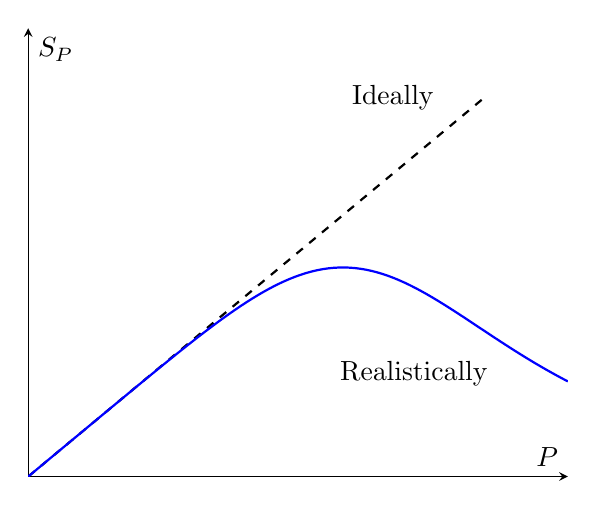
\begin{tikzpicture}
    \begin{axis}[
      xmin=0,
      xmax=1.3,
      ymin=0,
      ymax=1.3,
      axis lines=middle,
      ticks=none,
      xlabel={$P$},
      ylabel={$S_P$},
      ]
      \addplot[dashed, thick, domain=0:1.1, samples=100]{x};
      \addplot[blue, thick, domain=0:1.3, samples=100]{x/(1+x^5)};
      \node at (axis cs:1.0,1.1) [anchor=east] {Ideally};
      \node at (axis cs:1.13,0.3) [anchor=east] {Realistically};
    \end{axis}
  \end{tikzpicture}
  \caption{Ideal speedup ($S_P = P$) and realistic speedup: interpretation in terms of balance between local work and communication overhead.}
  \label{fig:scalability}
\end{figure}

$\rightarrow$ strong scaling should be interpreted carefully!

$\rightarrow$ weak scaling should also be considered.

\end{frame}


\begin{frame}
  \frametitle{Challenges of parallel computing}

Example Amdhal function for a node on Vilje: 16 processors
 
\begin{tikzpicture}[xscale=8,yscale=0.4,domain=0:1,samples=400]
      \draw[->] (0,0) -- (1,0) node[right] {$x$};
      \draw[->] (0,0) -- (0,16) node[above] {$y$};
      \draw[smooth,variable=\x,blue] plot ({\x},{16/(15*\x + 1)});
    \end{tikzpicture}

$\rightarrow$ steep decrease in efficiency
\end{frame}


\begin{frame}
  \frametitle{Performance scaling}

\medskip
\textbf{Amdahl's law}: relative speed-up
\begin{equation*}
S_p = \dfrac{1}{\dfrac{\alpha}{\bar S_p} + (1 - \alpha)}
\end{equation*}
with $\alpha$ fraction of time spent in \textbf{parallel} sections of the code.

\medskip
Example: How to reach $80$ percent of theoretical with $100$ processors?\\[2ex]
$\rightarrow$ less then $0.25$ should be spent in serial.

\medskip
$\rightarrow$ crucial to (re-)think algorithms for parallelism.

\end{frame}

\begin{frame}
  \frametitle{Communication cost}

\begin{itemize}
\item data movement between the different level of memory hierarchy
\item connections (bus, network) may exhibit hight latencies
\end{itemize}

\medskip
Latencies can be addressed by:
\begin{enumerate}
\item architectures: caching data.
\item software: rewriting data structures to improve locality.
\end{enumerate}

\medskip
The network communication is of order of a microsecond while cache latency is of order of a nanosecond:
\begin{equation*}
(1-\alpha) T_1 \approx T_c
\end{equation*}
with $T_c$ a communication cost.

\medskip
Linear model for communication: $Tc_(N) = T_s + N \gamma$
with $T_s$ an initialization latency and $\gamma$ a transmission speed (inverse bandwidth).
\end{frame}


\begin{frame}
  \frametitle{Relative performance}

\medskip
Relative speed-up analysis between two code versions
\begin{equation*}
S_p = \dfrac{T_1}{T_p} = \dfrac{p}{1 + p \dfrac{T_c}{T_1}}
\end{equation*}
with $T_c$ the communication time, if $T_c = 0$ ideal speed-up $S_p = p$.

\bigskip
Consider two versions of the same code with execution times:
\begin{equation*}
T_1^\ast << T_1
\end{equation*}
given for an optimized implementation $\ast$.

\medskip
Comparing $S_p$ and $S_p^\ast$
\begin{equation*}
\dfrac{S_p^\ast}{S_p} = \dfrac{1 + p \frac{T_c}{T_1}}{1 + p \frac{T_c}{T_1^\ast}}
\end{equation*}

\end{frame}

\begin{frame}
  \frametitle{Relative performance}

Comparing $S_p$ and $S_p^\ast$
\begin{equation*}
\dfrac{S_p^\ast}{S_p} = \dfrac{1 + p \frac{T_c}{T_1}}{1 + p \frac{T_c}{T_1^\ast}}
\end{equation*}

\medskip
\begin{equation*}
\frac{1}{T_1^\ast} > \frac{1}{T_1} \Rightarrow S_p^\ast < S_p
\end{equation*}

\medskip
The maximum speed-up for the optimized (faster) version is lower than the slow code: communication overhead is hidden.

\medskip
But, the optimized code remains faster!
\begin{equation*}
T_p^\ast = \frac{T_1^\ast}{p} + T_c
\end{equation*}
since $T_1^\ast << T_1$

\end{frame}

\begin{frame}
  \frametitle{Memory effect}

\medskip
Assume that the performance relation reads:
\begin{equation*}
T_p = \frac{T_1}{p} + T_c
\end{equation*}

\medskip
As before the first part consist of the cost of floating point operations and the second the cost of communication.

\medskip
Consider the operation rate when all the data can be stored in the cache: no memory latency
\begin{equation*}
T_1(\tau) = N \tau
\end{equation*}
for an optimal operation rate: $\tau$ is the average time spent for one floating-point operation.

\medskip
Consider the operation rate when some data needs to be fetched from the main memory
\begin{equation*}
T_1(\bar\tau) = N \bar\tau
\end{equation*}
with $\bar\tau = \tau + \mu$, $\mu$ the average penalty for fetch data from the main memory.

\end{frame}

\begin{frame}
  \frametitle{Memory effect}

\medskip
Assume that the performance relation reads:
\begin{equation*}
T_p(\tau) = \frac{T_1(\tau)}{p} + T_c = \frac{N \tau}{p} + T_c
\end{equation*}

\medskip
\begin{equation*}
S_p = \dfrac{T_1(\bar\tau)}{T_p(\tau)}
\end{equation*}

\medskip
\begin{equation*}
S_p = \dfrac{p}{\dfrac{\tau}{\bar\tau} + p \dfrac{T_c}{T_1(\bar\tau)}}
\end{equation*}

\medskip
If all the data fits in the cache then  $\tau = \bar\tau$, otherwise the speed can be super-linear: the explanation is that for big problems for low number of processes any access to the main memory will incur a penalty.


\end{frame}

\input{postamble}
